% -*- TeX-engine: xetex; eval: (auto-fill-mode 0); eval: (visual-line-mode 1); -*-
% Compile with XeLaTeX

%%%%%%%%%%%%%%%%%%%%%%%
% To do before class
%%%%%%%%%%%%%%%%%%%%%%%

% Send the Logistics/Week0Annoucnement (the night before).
% Send an email reminding students to bring a charged computer (the night before).

%%%%%%%%%%%%%%%%%%%%%%%
% Option 1: Slides: (comment for handouts)   %
%%%%%%%%%%%%%%%%%%%%%%%

\documentclass[slidestop,compress,mathserif,12pt,t,professionalfonts,xcolor=table]{beamer}

% solution stuff
\newcommand{\solnMult}[1]{
\only<1>{#1}
\only<2->{\red{\textbf{#1}}}
}
\newcommand{\soln}[1]{\textit{#1}}

\newcommand{\solnMultOn}[3]{
\only<#1>{#3}
\only<{#2}->{\red{\textbf{#3}}}
}

%%%%%%%%%%%%%%%%%%%%%%%%%%%%%%%
% Option 2: Handouts, without solutions (post before class)    %
%%%%%%%%%%%%%%%%%%%%%%%%%%%%%%%

% \documentclass[11pt,containsverbatim,handout,xcolor=xelatex,dvipsnames,table]{beamer}

% % handout layout
% \usepackage{pgfpages}
% \pgfpagesuselayout{4 on 1}[letterpaper,landscape,border shrink=5mm]

% % solution stuff
% \newcommand{\solnMult}[1]{#1}
% \newcommand{\soln}[1]{}
% \newcommand{\solnMultOn}[3]{#3}

% % % This breaks things for me for some reason.
% % tell pgfpages how to set page sizes in XeLaTeX
% %\renewcommand\pgfsetupphysicalpagesizes{%
% %   \pdfpagewidth\pgfphysicalwidth\pdfpageheight\pgfphysicalheight%
% %}

%%%%%%%%%%%%%%%%%%%%%%%%%%%%%%%%%%%%
% Option 3: Handouts, with solutions (may post after class if need be)    %
%%%%%%%%%%%%%%%%%%%%%%%%%%%%%%%%%%%%

% \documentclass[11pt,containsverbatim,handout,xcolor=xelatex,dvipsnames,table]{beamer}

% % handout layout
% \usepackage{pgfpages}
% \pgfpagesuselayout{4 on 1}[letterpaper,landscape,border shrink=5mm]

% % solution stuff
% \newcommand{\solnMult}[1]{\red{\textbf{#1}}}
% \newcommand{\soln}[1]{\textit{#1}}

% % % This breaks things for me for some reason.
% % % tell pgfpages how to set page sizes in XeLaTeX
% % \renewcommand\pgfsetupphysicalpagesizes{%
% %    \pdfpagewidth\pgfphysicalwidth\pdfpageheight\pgfphysicalheight%
% % }

%%%%%%%%%%%%%%%%%%%%%%%%%%%%%%%
% Option 4: Notes Only
%%%%%%%%%%%%%%%%%%%%%%%%%%%%%%%

% % See http://tex.stackexchange.com/questions/114219/add-notes-to-latex-beamer
% \documentclass[10pt,containsverbatim,xcolor=xelatex,dvipsnames,table,notes=only]{beamer}

% % handout layout
% % \usepackage{pgfpages}
% % \pgfpagesuselayout{1 on 1}[letterpaper, landscape, border shrink=5mm]

% % solution stuff
% \newcommand{\solnMult}[1]{#1}
% \newcommand{\soln}[1]{}

% % % Having a problem with this.
% % tell pgfpages how to set page sizes in XeLaTeX
% % \renewcommand\pgfsetupphysicalpagesizes{%
% %   \pdfpagewidth\pgfphysicalwidth\pdfpageheight\pgfphysicalheight%
% %}

%%%%%%%%%%
% Load style file, defaults  %
%%%%%%%%%%

%%%%%%%%%%%%%%%%
% Themes
%%%%%%%%%%%%%%%%

% See http://deic.uab.es/~iblanes/beamer_gallery/ for mor options

% Style theme
\usetheme{Pittsburgh}

% Color theme
\usecolortheme{seahorse}

% Font theme
%\usepackage[T1]{fontenc}
%\usepackage[scaled=0.92]{helvet}

%\usepackage[no-math]{fontspec}
%\setsansfont{TeX Gyre Heros}
% "TeX Gyre Heros can be used as a replacement for Helvetica"
% In Unix, unzip the following into ~/.fonts
% In Mac, unzip it, double-click the .otf files, and install using "FontBook"
%   http://www.gust.org.pl/projects/e-foundry/tex-gyre/heros/qhv2.004otf.zip

\usepackage{fontspec}

%%%%%%%%%%%%%%%%
% Packages
%%%%%%%%%%%%%%%%

\usepackage{geometry}
\usepackage{graphicx}
\usepackage{amssymb}
\usepackage{epstopdf}
\usepackage{amsmath}  	% this permits text in eqnarray among other benefits
\usepackage{url}		% produces hyperlinks
\usepackage[english]{babel}
\usepackage[latin1]{inputenc}
\usepackage{colortbl}	% allows for color usage in tables
\usepackage{multirow}	% allows for rows that span multiple rows in tables
\usepackage{color}		% this package has a variety of color options
\usepackage{colortbl}
\usepackage{pgf}
\usepackage{calc}
\usepackage{ulem}
\usepackage{multicol}
\usepackage{textcomp}
\usepackage{txfonts}
\usepackage{listings}
\usepackage{tikz}
\usepackage{fancyvrb}

%%%%%%%%%%%%%%%%
% Remove navigation symbols
%%%%%%%%%%%%%%%%

\beamertemplatenavigationsymbolsempty
\hypersetup{pdfpagemode=UseNone} % don't show bookmarks on initial view

%%%%%%%%%%%%%%%%
% User defined colors
%%%%%%%%%%%%%%%%

% Pantone 2015 Spring colors
% http://iwork3.us/2014/09/16/pantone-2015-spring-fashion-report/
% update each semester or year

\xdefinecolor{custom_blue}{rgb}{0, 0.70, 0.79} % scuba blue
\xdefinecolor{custom_darkBlue}{rgb}{0.11, 0.31, 0.54} % classic blue
\xdefinecolor{custom_orange}{rgb}{0.97, 0.57, 0.34} % tangerine
\xdefinecolor{custom_green}{rgb}{0.49, 0.81, 0.71} % lucite green
\xdefinecolor{custom_red}{rgb}{0.58, 0.32, 0.32} % marsala

\xdefinecolor{custom_lightGray}{rgb}{0.78, 0.80, 0.80} % glacier gray
\xdefinecolor{custom_darkGray}{rgb}{0.54, 0.52, 0.53} % titanium

%%%%%%%%%%%%%%%%
% Template colors
%%%%%%%%%%%%%%%%

\setbeamercolor*{palette primary}{fg=white,bg= custom_blue}
\setbeamercolor*{palette secondary}{fg=black,bg= custom_blue!80!black}
\setbeamercolor*{palette tertiary}{fg=white,bg= custom_blue!80!black!80}
\setbeamercolor*{palette quaternary}{fg=white,bg= custom_blue}

\setbeamercolor{structure}{fg= custom_blue}
\setbeamercolor{frametitle}{bg= custom_blue!90}
\setbeamertemplate{blocks}[shadow=false]
\setbeamersize{text margin left=2em,text margin right=2em}

%%%%%%%%%%%%%%%%
% Styling fonts, bullets, etc.
%%%%%%%%%%%%%%%%

% styling of itemize bullets
\setbeamercolor{item}{fg=custom_blue}
\setbeamertemplate{itemize item}{{{\small$\blacktriangleright$}}}
\setbeamercolor{subitem}{fg=custom_blue}
\setbeamertemplate{itemize subitem}{{\textendash}}
\setbeamerfont{itemize/enumerate subbody}{size=\footnotesize}
\setbeamerfont{itemize/enumerate subitem}{size=\footnotesize}

% styling of enumerate bullets
\setbeamertemplate{enumerate item}{\insertenumlabel.}
\setbeamerfont{enumerate item}{family={\fontspec{Helvetica Neue}}}
\setbeamerfont{enumerate subitem}{family={\fontspec{Helvetica Neue}}}
\setbeamerfont{enumerate subsubitem}{family={\fontspec{Helvetica Neue}}}

% make frame titles small to make room in the slide
\setbeamerfont{frametitle}{size=\small} 

% set Helvetica Neue font for frame and section titles
\setbeamerfont{frametitle}{family={\fontspec{Helvetica Neue}}}
\setbeamerfont{sectiontitle}{family={\fontspec{Helvetica Neue}}}
\setbeamerfont{section in toc}{family={\fontspec{Helvetica Neue}}}
\setbeamerfont{subsection in toc}{family={\fontspec{Helvetica Neue}}, size=\small}
\setbeamerfont{footline}{family={\fontspec{Helvetica Neue}}}
\setbeamerfont{subsection in toc}{family={\fontspec{Helvetica Neue}}}
\setbeamerfont{block title}{family={\fontspec{Helvetica Neue}}}

%%%%%%%%%%%%%%%%
% Color text commands
%%%%%%%%%%%%%%%%

%orange
\newcommand{\orange}[1]{\textit{\textcolor{custom_orange}{#1}}}

% green
\newcommand{\green}[1]{\textit{\textcolor{custom_green}{#1}}}

% red
\newcommand{\red}[1]{\textit{\textcolor{custom_red}{#1}}}

% dark gray
\newcommand{\darkgray}[1]{\textit{\textcolor{custom_darkGray}{#1}}}

% light gray
\newcommand{\lightgray}[1]{\textit{\textcolor{custom_lightGray}{#1}}}


%%%%%%%%%%%%%%%%
% Custom commands
%%%%%%%%%%%%%%%%

% cancel
\newcommand{\cancel}[1]{%
    \tikz[baseline=(tocancel.base)]{
        \node[inner sep=0pt,outer sep=0pt] (tocancel) {#1};
        \draw[red, line width=0.5mm] (tocancel.south west) -- (tocancel.north east);
    }%
}

% degree
\newcommand{\degree}{\ensuremath{^\circ}}

% cite
\newcommand{\ct}[1]{
\vfill
{\tiny #1}}

% Note
\newcommand{\Note}[1]{
\rule{2.5cm}{0.25pt} \\ \textit{\footnotesize{\textcolor{custom_red}{Note:} \textcolor{custom_darkGray}{#1}}}}

% Remember
\newcommand{\Remember}[1]{\textit{\scriptsize{\textcolor{custom_red}{Remember:} #1}}}

% links: webURL, webLink
\newcommand{\webURL}[1]{\urlstyle{same}{\textit{\textcolor{custom_blue}{\url{#1}}}}}
\newcommand{\webLink}[2]{\href{#1}{\textcolor{custom_blue}{{#2}}}}

% mail
\newcommand{\mail}[1]{\href{mailto:#1}{\textit{\textcolor{custom_blue}{#1}}}}

% highlighting: hl, hlGr, mathhl
\newcommand{\hl}[1]{\textit{\textcolor{custom_blue}{#1}}}
\newcommand{\hlGr}[1]{\textit{\textcolor{custom_green}{#1}}}
\newcommand{\mathhl}[1]{\textcolor{custom_blue}{\ensuremath{#1}}}

% example
\newcommand{\ex}[1]{\textcolor{blue}{{{\small (#1)}}}}

% two col: two columns
\newenvironment{twocol}[4]{
\begin{columns}[c]
\column{#1\textwidth}
#3
\column{#2\textwidth}
#4
\end{columns}
}

% slot (for probability calculations)
\newenvironment{slot}[2]{
\begin{array}{c} 
\underline{#1} \\ 
#2
\end{array}
}

% pr: left and right parentheses
\newcommand{\pr}[1]{
\left( #1 \right)
}

%%%%%%%%%%%%%%%%
% Custom blocks
%%%%%%%%%%%%%%%%

% activity: less commonly used
\newcommand{\activity}[2]{
\setbeamertemplate{itemize item}{{{\small\textcolor{custom_orange}{$\blacktriangleright$}}}}
\setbeamercolor{block title}{fg=white, bg=custom_orange}
\setbeamerfont{block title}{size=\small}
\setbeamercolor{block body}{fg=black, bg=custom_orange!20!white!80}
\setbeamerfont{block body}{size=\small}
\begin{block}{Activity: #1}
#2
\end{block}
}

% app: application exercise
\newcommand{\app}[2]{
\setbeamercolor{block title}{fg=white,bg=custom_green}
\setbeamercolor{block body}{fg=black,bg=custom_green!20!white!80}
\begin{block}{{\small Application exercise: #1}}
#2
\end{block}
}

% disc: discussion question
\newcommand{\disc}[1]{
\setbeamercolor{block body}{bg=custom_blue!25!white!80, fg=custom_blue!55!black!95}
\begin{block}{\vspace*{-3ex}}
#1
\end{block}
}

% clicker: clicker question
\newcommand{\clicker}[1]{
\setbeamercolor{block title}{bg=custom_blue!80!white!50,fg=custom_blue!30!black!90}
\setbeamercolor{block body}{bg=custom_blue!20!white!80,fg=custom_blue!30!black!90}
\begin{block}{\vspace*{-0.2ex}{\footnotesize Clicker question}\vspace*{-0.2ex}}
#1
\end{block}
}

% formula
\newcommand{\formula}[2]{
\setbeamercolor{block title}{bg=custom_blue!40!white!60,fg=custom_blue!55!black!95}
\begin{block}{{\small#1}}
#2
\end{block}
}

% code
\newcommand{\code}[1]{
\newfontfamily{\monaco}{Monaco}
{\monaco {\footnotesize \textcolor{custom_darkBlue}{#1}}}
}

% output
\renewcommand{\output}[1]{
{\monaco {\footnotesize \textcolor{custom_darkGray}{#1}}}
}

%%%%%%%%%%%%%%%%
% Change margin
%%%%%%%%%%%%%%%%

\newenvironment{changemargin}[2]{%
\begin{list}{}{%
\setlength{\topsep}{0pt}%
\setlength{\leftmargin}{#1}%
\setlength{\rightmargin}{#2}%
\setlength{\listparindent}{\parindent}%
\setlength{\itemindent}{\parindent}%
\setlength{\parsep}{\parskip}%
}%
\item}{\end{list}}

%%%%%%%%%%%%%%%%
% Footnote
%%%%%%%%%%%%%%%%

\long\def\symbolfootnote[#1]#2{\begingroup%
\def\thefootnote{\fnsymbol{footnote}}\footnote[#1]{#2}\endgroup}

%%%%%%%%%%%%%%%%
% Graphics
%%%%%%%%%%%%%%%%

\DeclareGraphicsRule{.tif}{png}{.png}{`convert #1 `dirname #1`/`basename #1 .tif`.png}

%%%%%%%%%%%%%%%%
% Slide number
%%%%%%%%%%%%%%%%

\setbeamertemplate{footline}{%
    \raisebox{5pt}{\makebox[\paperwidth]{\hfill\makebox[20pt]{\color{gray}
          \scriptsize\insertframenumber}}}\hspace*{5pt}}

          
%%%%%%%%%%%%%%%%
% Remove page numbers
%%%%%%%%%%%%%%%%

\newcommand{\removepagenumbers}{% 
  \setbeamertemplate{footline}{}
}

%%%%%%%%%%%%%%%%
% TOC slides
%%%%%%%%%%%%%%%%

% TRY TO CHANGE THE ENUMERATE SYMBOLS HERE FROM CIRCLES TO PLAIN NUMBERS

\AtBeginSection[] 
{ 
  \addtocounter{framenumber}{-1} 
  % 
  {\removepagenumbers 
    \begin{frame}<beamer> 
    \tableofcontents[currentsection] 
  \end{frame} 
  } 
}
% You cannot use numbers when defining variables.  Hence the use of letters, A, B, C, etc.

% Personal Info
\newcommand{\FirstName}{Mine}
\newcommand{\LastName}{\c{C}etinkaya-Rundel}
\newcommand{\OfficeHours}{MTWR 3-4pm.}
\newcommand{\OfficeHoursLocation}{Old Chem 213}

% Electronic Info
\newcommand{\PersonalSite}{http://stat.duke.edu/~mc301}
\newcommand{\CourseSite}{http://bitly.com/sta101sp15}
\newcommand{\Email}{mine@stat.duke.edu}

% TAs
\newcommand{\TAA}{Anthony Weishampel}
\newcommand{\TAB}{Fiamma Li}
\newcommand{\TAC}{Jialiang Mao}
\newcommand{\TAD}{Phillip Lee}

% Exam Dates
\newcommand{\ExamADate}{Wed, Feb 18}
\newcommand{\ExamBDate}{Wed, Mar 25}
\newcommand{\FinalDate}{Sat, May 2 (2-5pm)}

% Due Dates
\newcommand{\ClickerRegistrationDD}{Mon, Jan 26}
\newcommand{\GettingToKnowYouDD}{Friday, Jan 9, 11:59pm}
\newcommand{\ProblemSetADD}{Wed., 1/15}


% ALT ALT
% You cannot use numbers when defining variables.  Hence the use of letters, A, B, C, etc.

% Personal Info
\renewcommand{\FirstName}{Jesse}
\renewcommand{\LastName}{Windle}
\renewcommand{\OfficeHours}{Tue, Thu 3:00pm-4:30pm}

% Electronic Info
\renewcommand{\PersonalSite}{http://stat.duke.edu/~jbw44/}
\renewcommand{\CourseSite}{http://bitly.com/windle2}
\renewcommand{\Email}{jbw44@stat.duke.edu}

% TAs
\renewcommand{\TAA}{David Clancy}
\renewcommand{\TAB}{Xinyi (Chris) Li}
\renewcommand{\TAC}{Tori Hall}
\renewcommand{\TAD}{Radhika Anand}

% Exam Dates
\renewcommand{\ExamADate}{Thu, Feb 19}
\renewcommand{\ExamBDate}{Thu, Mar 26}
\renewcommand{\FinalDate}{Mon, Apr 27 (9-Noon)}

% Due Dates
\renewcommand{\ClickerRegistrationDD}{Thu, Jan 15}
\renewcommand{\GettingToKnowYouDD}{Friday, Jan 9, 11:59pm}

%%%%%%%%%%%
% Cover slide info    %
%%%%%%%%%%%

\title{Unit 4: Inference for numerical data}
\subtitle{3. ANOVA}
\author{Sta 101 - Spring 2015}
\date{March 4, 2015}
\institute{Duke University, Department of Statistical Science}

%%%%%%%%%%%
% Main ideas %
%%%%%%%%%%%

\newcommand{\mainideaA}{You can use the $F$-test to compare grouping by 2 variables vs. grouping by 1 variable}

\newcommand{\bonferroni}{If you want to test many hypotheses simulteneously, use
  the Bonferroni correction.}

%%%%%%%%%%%
% Begin document   %
%%%%%%%%%%%

\begin{document}

%%%%%%%%%%%%%%%%%%%%%%%%%%%%%%%%%%%%

% Title Page

\begin{frame}[plain]

\titlepage
\vfill
{\scriptsize \webLink{\PersonalSite}{Dr. \LastName{}} \hfill Slides posted at  \webLink{\CourseSite}{\CourseSite}}
\addtocounter{framenumber}{-1} 

\end{frame}

%%%%%%%%%%%%%%%%%%%%%%%%%%%%%%%%%%%%

\section{Housekeeping}

%%%%%%%%%%%%%%%%%%%%%%%%%%%%%%%%%%%%

\begin{frame}
\frametitle{Announcements}

\begin{itemize}

\item 

\end{itemize}

\end{frame}

%%%%%%%%%%%%%%%%%%%%%%%%%%%%%%%%%%%%

\section{Main Ideas}

% %%%%%%%%%%%%%%%%%%%%%%%%%%%%%%%%%%%%

% \subsection{\bonferroni}
% \label{mi1}

% %%%%%%%%%%%%%%%%%%%%%%%%%%%%%%

% \begin{frame}
%   \frametitle{Last time}

%   \vfill

%   \url{http://imgs.xkcd.com/comics/significant.png}

%   \vfill

% \end{frame}

% %%%%%%%%%%%%%%%%%%%%%%%%%%%%%%

% \begin{frame}
%   \frametitle{Last time}

%   \textbf{Suppose} $\alpha = 0.05$.

%   \disc{What is the probability of correctly failing to reject
%     \[
%     H_0: \mu_{\textmd{purple}} = \mu_{\textmd{placebo}} \; ?
%     \]
%     }

%     \pause

%     \hfill \\

%     \clicker{If all the tests are independent and if no color of Jelly bean has any link to acne, what is the
%       probability of making at least one type I error in the 20 trials?}
%       \begin{enumerate}[(a)]
%       \item 5\%
%       \item 36\%
%       \item \solnMultOn{2}{3}{64\%}
%       \item 95\%
%       \end{enumerate}

% \end{frame}

% %%%%%%%%%%%%%%%%%%%%%%%%%%%%%%

% \begin{frame}
%   \frametitle{Last Time}

% Is some jelly bean linked to acne?  Use the $F$-test.

% \begin{itemize}
% \item $H_0$: the placebo and all of the jelly beans have the same group means.

% \item $H_A$: at least one of the group's has a mean that is different from the others.
% \end{itemize}

% \clicker{For the $F$-test, what is the probability of incorrectly rejecting the null?}
% \begin{enumerate}[(a)]
% \item \solnMult{5\%}
% \item 36\%
% \item 64\%
% \item 95\%
% \end{enumerate}

% \end{frame}

% %%%%%%%%%%%%%%%%%%%%%%%%%%%%%%

% \begin{frame}
%   \frametitle{The Bonferroni correction}

%   \vfill 

%   \disc{How do we figure out \emph{which} jelly bean(s) is(are) linked to acne?}

%   \begin{center}
%   The Bonferroni correction.
%   \end{center}

%   \vfill

% \end{frame}

% %%%%%%%%%%%%%%%%%%%%%%%%%%%%%%

% \begin{frame}
%   \frametitle{1. \bonferroni}

% \vfill

% Bonferroni correction: 
% \begin{itemize}
% \item Target type I error rate: $\alpha$.

% \item Number of null/alt hypotheses to be tested using the same data set: $K$

% \item If you set the significance level for each test to be
% \[
% \alpha^* = \alpha / K,
% \]
% then the probability of making one or more type I errors is $ \leq \alpha$.

% \end{itemize}

% \vfill

% \end{frame}

% %%%%%%%%%%%%%%%%%%%%%%%%%%%%%%

% \begin{frame}
%   \frametitle{1. \bonferroni}

% \vspace{-0.5cm}
% {\small
% \begin{align*}
% 01.\ &  \; \; H_0: \; \mu_{\text{placebo}} = \mu_{\text{purple}} \\
%      &  \; \; H_A: \; \mu_{\text{placebo}} \neq \mu_{\text{purple}}  \\
% 02.\ &  \; \; H_0: \; \mu_{\text{placebo}} = \mu_{\text{brown}} \\
%      &  \; \; H_A: \; \mu_{\text{placebo}} \neq \mu_{\text{brown}}  \\
% & \ldots \\
% % 19.\ &  \; \; H_0: \; \mu_{\text{placebo}} = \mu_{\text{peach}} \\
% %      &  \; \; H_A: \; \mu_{\text{placebo}} \neq \mu_{\text{peach}}  \\
% 20.\ &  \; \; H_0: \; \mu_{\text{placebo}} = \mu_{\text{orange}} \\
%      &  \; \; H_A: \; \mu_{\text{placebo}} \neq \mu_{\text{orange}} 
% \end{align*}
% }

% \clicker{What significance level shoud we use to test all of these hypotheses simultaneously for a type I error rate of 5\%?}
% \begin{center}
% (a) 0.0024 \; (b) \solnMult{0.0025} (c) 0.0026 \; (d) 0.05
% \end{center}

% \end{frame}

% %%%%%%%%%%%%%%%%%%%%%%%%%%%%%%

% \begin{frame}
%   \frametitle{1. \bonferroni}

% \vfill

% \app{4.5 ANOVA - Pt 2}{See the course webpage for details.}

% \vfill

% \end{frame}


% %%%%%%%%%%%%%%%%%%%%%%%%%%%%%%%%%%%%

% \subsection{\mainideaA}
% \label{mi1}

% %%%%%%%%%%%%%%%%%%%%%%%%%%%%%%%%%%%%

% \begin{frame}
%   \frametitle{2. \mainideaA}

%   Cartoon for incorporating cholcolate.

%   Jelly beans are associated with Acne.
%   OK.
%   I hear chocholate makes it works.

% \end{frame}

% %%%%%%%%%%%%%%%%%%%%%%%%%%%%%%%%%%%%

% \begin{frame}
%   \frametitle{2. \mainideaA}

%   Treatments:

%   \begin{center}
%   \begin{tabular}{l l}
%     purple \& choc.\ & purple \& no choc. \\
%     brown \& choc.\ & brown \& no choc. \\
%     \ldots & \ldots \\
%     orange \& chol.\ & orange \& no choc.
%     \end{tabular}
%     \end{center}

%     \clicker{We want to test if eating chocolate and a certain color jelly bean has a different impact than just eating that color jelly bean.  Which type of null hypothesis should we use?}
%     \begin{enumerate}[(a)]
%       \item $H_0$: $\mu_{\textmd{color \& choc.}} = \mu_{\textmd{color \& no choc.}}$ for every color.
%       \item $H_0$: $\mu_{\textmd{color A \& choc.}} = \mu_{\textmd{color B \& choc.}}$ for every pair of colors.
%       \end{enumerate}

% \end{frame}

% %%%%%%%%%%%%%%%%%%%%%%%%%%%%%%%%%%%%

% \begin{frame}
%   \frametitle{2. \mainideaA}

% Picture of within group variation for different scenarios.

% \end{frame}

% %%%%%%%%%%%%%%%%%%%%%%%%%%%%%%%%%%%%

% \begin{frame}
%   \frametitle{2. \mainideaA}

%   $F$-test in terms of difference of within group variation.

% \end{frame}

% %%%%%%%%%%%%%%%%%%%%%%%%%%%%%%%%%%%%

% \begin{frame}
%   \frametitle{2. \mainideaA}

%   App Ex.

% \end{frame}


%%%%%%%%%%%%%%%%%%%%%%%%%%%%%%%%%%%%%%%%%%%%%%%%%%%%%%%%%%%%%%%%%%%%%%%%%%%%%%%%
%%%%%%%%%%%%%%%%%%%%%%%%%%%%%%%%%%%%%%%%%%%%%%%%%%%%%%%%%%%%%%%%%%%%%%%%%%%%%%%%
%%%%%%%%%%%%%%%%%%%%%%%%%%%%%%%%%%%%%%%%%%%%%%%%%%%%%%%%%%%%%%%%%%%%%%%%%%%%%%%%

%%%%%%%%%%%%%%%%%%%%%%%%%%%%%%%%%%

\subsection{\bonferroni}

\begin{frame}
  \frametitle{ANOVA Review}

\vfill

An example by James G. Scott:
\begin{quote} 
[These data are] from an experiment run by a British video-game manufacturer in an attempt to calibrate the level of difficulty of certain tasks in the video game. Subjects in this experiment were presented with a simple “Where’s Waldo?”-style visual scene. The subjects had to find a number (1 or 2) floating somewhere in the scene, to identify the number, and to press the corresponding button as quickly as possible. The response variable is their reaction time.
\end{quote}

\vfill

\end{frame}

%%%%%%%%%%%%%%%%%%%%%%%%%%%%%%%%%%

\begin{frame}[fragile]
  \frametitle{ANOVA Review}
  
\begin{center}
{\small
\begin{verbatim}
Obs  Subject PictureTarget.RT Littered FarAway
  1       10              635        0       0
  2       10             1144        0       0
  3       10              570        0       0
  4       10              589        0       0
  5       10              754        0       0
  6       10              601        0       0
\end{verbatim}
}
\end{center}

\small
{\tiny From JGS:}
\begin{itemize}
\item \texttt{PictureTarget.RT}: the subject’s reaction time in milliseconds.
\item \texttt{Subject}: a numerical identifier for the subject undergoing the test.
\item \texttt{FarAway}: was the number to be identified far away (1) or near (0) in the visual scene?
\item \texttt{Littered}: the British way of saying whether the scene was cluttered (1) or mostly free of clutter (0).
\end{itemize}

\end{frame}


%%%%%%%%%%%%%%%%%%%%%%%%%%%%%%%%%%

\begin{frame}
  \frametitle{ANOVA Review}

  \disc{Do some subjects in the study have different mean reaction times?}

  \begin{center}
  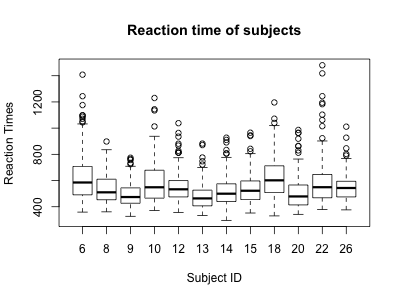
\includegraphics[scale=0.6]{figures/rxntime-boxplots.png}
  \end{center}

\end{frame}


%%%%%%%%%%%%%%%%%%%%%%%%%%%%%%%%%%

\begin{frame}[fragile]
  \frametitle{ANOVA Review}

Number of observations $n = 1920$.

\hfill \\

{\small
ANOVA Table
\begin{verbatim}
              Df   Sum Sq  Mean Sq  Fvalue    Pr(>F)    
Subject       ??  4060822   369166    20.5   2.2e-16
Residuals     ?? 35129401    18412
\end{verbatim}
}

% Response: PictureTarget.RT
%                      Df   Sum Sq Mean Sq F value    Pr(>F)    
% as.factor(Subject)   11  4060822  369166  20.051 < 2.2e-16 ***
% Residuals          1908 35129401   18412 

\clicker{What are the degrees of freedom?}
\begin{enumerate}[(a)]
\item  1 and 1909
\item \solnMult{11 and 1908}
\item 11 and 1909
\item 12 and 1908
\end{enumerate}

\end{frame}

%%%%%%%%%%%%%%%%%%%%%%%%%%%%%%%%%%

\begin{frame}[fragile]
  \frametitle{ANOVA Review}

  \clicker{What is the most appropriate conclusion?}
  \begin{enumerate}[(a)]
  \item There is no evidence that the subjects have different mean reaction times.
  \item There is no evidence that some of the subjects have the same mean reaction times.
  \item \solnMult{Some pairs of subjects have different mean reaction times.}
  \item All paris of subjects have different mean reaction times.
  \end{enumerate}

\end{frame}

%%%%%%%%%%%%%%%%%%%%%%%%%%%%%%

\begin{frame}
  \frametitle{The Bonferroni correction}

  \vfill 

  \disc{How do we determine which subjects have a different mean reaction time than Subject 6?}

  \begin{center}
  The Bonferroni correction.
  \end{center}

  \vfill

\end{frame}


%%%%%%%%%%%%%%%%%%%%%%%%%%%%%%

\begin{frame}
  \frametitle{The Bonferroni correction}

Goal: test 11 different hypotheses:

{\small
\begin{align*}
01.\ &  \; \; H_0: \; \mu_{\text{S06}} = \mu_{\text{S08}} \\
     &  \; \; H_A: \; \mu_{\text{S06}} \neq \mu_{\text{S08}}  \\
02.\ &  \; \; H_0: \; \mu_{\text{S06}} = \mu_{\text{S09}} \\
     &  \; \; H_A: \; \mu_{\text{S06}} \neq \mu_{\text{S09}}  \\
& \ldots \\
11.\ &  \; \; H_0: \; \mu_{\text{placebo}} = \mu_{\text{S26}} \\
     &  \; \; H_A: \; \mu_{\text{placebo}} \neq \mu_{\text{S26}} 
\end{align*}
}

\emph{AND} keep the Type I error rate at or below the significance level.

\end{frame}

%%%%%%%%%%%%%%%%%%%%%%%%%%%%%%

\begin{frame}
  \frametitle{1. \bonferroni}

\vfill

Bonferroni correction: 
\begin{itemize}
\item Target type I error rate: $\alpha$.

\item Number of null/alt hypotheses to be tested using the same data set: $K$

\item If you set the significance level for each test to be
\[
\alpha^* = \alpha / K,
\]
then the probability of making one or more type I errors is $ \leq \alpha$.

\end{itemize}

\vfill

\end{frame}

%%%%%%%%%%%%%%%%%%%%%%%%%%%%%%

\begin{frame}[fragile]
  \frametitle{1. \bonferroni}

\begin{minipage}{0.3\textwidth}
\small
\begin{verbatim}
Hyp   p-value
 01  4.27e-09 
 02   < 2e-16 
 03   0.00368 
 04  5.68e-07 
 05   < 2e-16 
 06  1.82e-13 
 07  1.11e-09 
 08   0.61587    
 09  1.42e-14 
 10   0.02332 
 11  1.91e-07 
\end{verbatim}
\end{minipage}%
\begin{minipage}{0.6\textwidth}
\clicker{Which null hypotheses should we reject at $\alpha = 0.05$?}
\begin{enumerate}[(a)]
\item 1, 2, 3, 4, 5, 6, 7, 8, 9, 10, 11
\item \solnMult{1, 2, 3, 4, 5, 6, 7,    9,     11}
\item 1, 2,    4, 5, 6, 7,    9,     11
\item 1, 2,       5, 6, 7,    9,     11
\end{enumerate}
\end{minipage}

\end{frame}


%%%%%%%%%%%%%%%%%%%%%%%%%%%%%%

\begin{frame}
  \frametitle{1. \bonferroni}

\vfill

\app{4.5 ANOVA - Pt 2}{See the course webpage for details.}

\vfill

\end{frame}

%%%%%%%%%%%%%%%%%%%%%%%%%%%%%%

\subsection{\mainideaA}

\begin{frame}
  \frametitle{\mainideaA}

A new research question:

\disc{
Does "litter" in the image change some subjects' reaction times?
}

{\small
\begin{align*}
01.\ &  \; \; H_0: \; \mu_{\text{S06 \& Litter}} = \mu_{\text{S06 \& No Litter}} \\
     &  \; \; H_A: \; \mu_{\text{S06 \& Litter}} \neq \mu_{\text{S06 \& No Litter}} \\
02.\ &  \; \; H_0: \; \mu_{\text{S08 \& Litter}} = \mu_{\text{S08 \& No Litter}} \\
     &  \; \; H_A: \; \mu_{\text{S08 \& Litter}} \neq \mu_{\text{S08 \& No Litter}} \\
     & \ldots \\
12.\ &  \; \; H_0: \; \mu_{\text{S26 \& Litter}} = \mu_{\text{S26 \& No Litter}} \\
     &  \; \; H_A: \; \mu_{\text{S26 \& Litter}} \neq \mu_{\text{S26 \& No Litter}} 
\end{align*}
}

Same problem as before... multpile hypotheses.

\end{frame}

%%%%%%%%%%%%%%%%%%%%%%%%%%%%%%%%%%

\begin{frame}
  \frametitle{\mainideaA}

Null hypothesis: litter does not change the mean reaction time of anyone.

\hspace \\


{\small
\begin{align*}
H_0: \; & \mu_{\text{S06 \& Litter}} = \mu_{\text{S06 \& No Litter}} \\
\textmd{and } \; & \mu_{\text{S08 \& Litter}} = \mu_{\text{S08 \& No Litter}} \\
\textmd{and } \; & \; \; \; \ldots \\
\textmd{and } \; & \mu_{\text{S26 \& Litter}} = \mu_{\text{S26 \& No Litter}} \\
\end{align*}
}

\end{frame}

%%%%%%%%%%%%%%%%%%%%%%%%%%%%%%%%%%

\section{Summary}

%%%%%%%%%%%%%%%%%%%%%%%%%%%%%%%%%%%%

\begin{frame}
\frametitle{Summary of main ideas}

\vfill

\begin{enumerate}

\item \nameref{mi1}

\end{enumerate}

\vfill

\end{frame}

%%%%%%%%%%%%%%%%%%%%%%%%%%%%%%%%%%%

\end{document}